\subsection{联合嵌入模型}
联合嵌入模型先将视觉信息和问题文本信息分别特征化,再通过特征向量串联\citing{zhou2015simple}、卷积\citing{ma2016learning}、逐元素相乘\citing{antol2015vqa}、逐元素相加\citing{malinowski2015ask}等池化方法融合图像特征和文本特征,最终得到最优答案。

Malinowski等人首次提出了应用于真实场景视觉问答任务的联合嵌入模型Neural-Image-QA
\citing{malinowski2015ask}。Neural-Image-QA是一个由卷积神经网络CNN和长短期记忆LSTM组成的深度网络,先使用在ImageNet预处理过的卷积神经网络CNN对图像进行特征提取,得到的特征向量和问题文本一起传输到长短期记忆LSTM中,从而生成答案的单词序列。模型在DAQUAR数据集上完成训练和测试,对于答案只有一个词语的问题,准确率为19.43\%,对于答案是多个词语的问题,准确率为17.49\%。不同于Malinowski的Neural-Image-QA,Gao等人认为问题和答案在句法结构上有所不同,因此编码问题的LSTM和解码答案的LSTM为采用两个独立的网络,使用不用的权重矩阵,结合卷积神经网络CNN构成了mQA模型\citing{NIPS2015_5641}。

Noh等人认为单单使用相同权重参数的深度卷积神经网络去处理不同的问题,并期待能得到足够准确的答案,这是很困难的\citing{noh2016image}。因此他们提出DPPnet,在卷积神经网络CNN中添加一个动态参数层,动态参数层中的参数会根据问题的不同而改变,这使得每个问题输入都对应一个独特的分类网络。模型由三个部分组成,一个部分作为分类网络的卷积神经网络,第二个部分是参数预测网络,由门控复发单位编码问题序列,再通过一个全连接层输入动态参数,第三个部分是一个哈希函数,将参数预测网络输出的动态参数配置到分类网络中。如图\ref{DP-CNN}。
\begin{figure}[H]
	\centering
	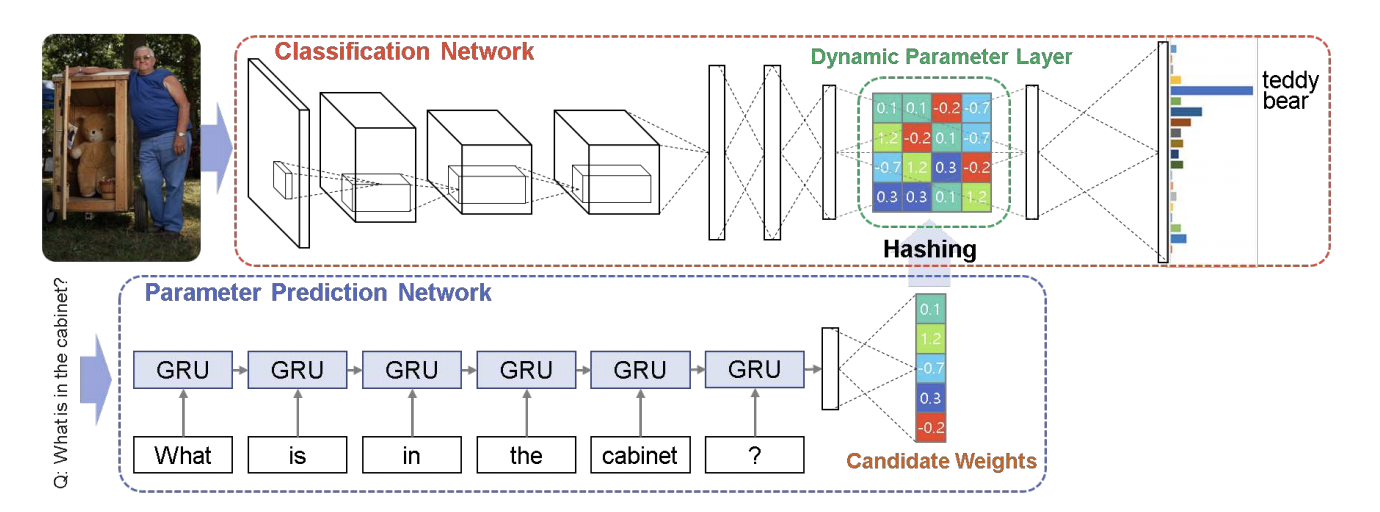
\includegraphics[width=0.8\textwidth]{DP-CNN.png}
	\caption{带有动态参数层的卷积网络模型DPPnet}
	\label{DP-CNN}
\end{figure}

Zhou等人同样适用预处理后的卷积神经网络CNN,但在处理问题文本时选择了比长短期记忆LSTM更为简单的词袋模型BOW,提出了iBOWIMG模型\citing{zhou2015simple}。iBOWIMG模型受到BOWIMG\citing{antol2015vqa}在VQA数据集上优于部分基于长短期记忆LSTM模型的启发,在原有基础上将VGGNet替换为在图像特征提取表现更优的GoogLeNet\citing{Szegedy_2015_CVPR},将图像特征向量和文本特征向量串联后送入softmax层预测问题答案(如图\ref{iBOWIMG}),在COCO-VQA数据集上的测试展现出具有竞争力的表现。
\begin{figure}[H]
	\centering
	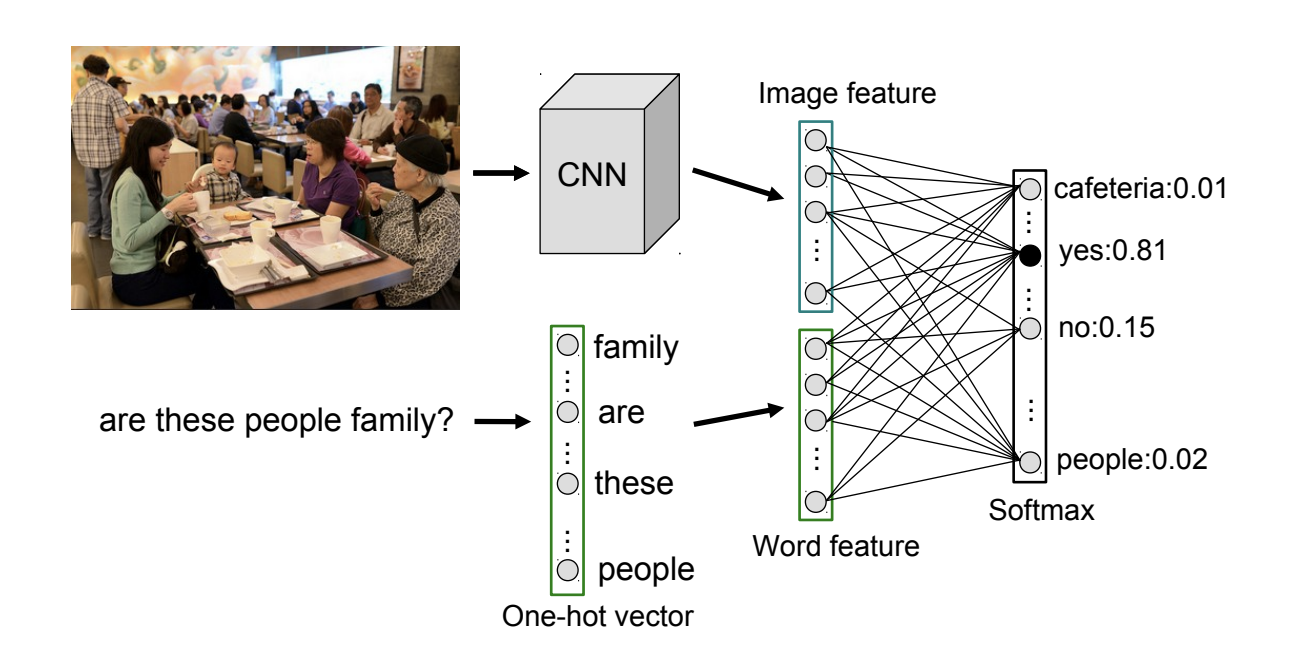
\includegraphics[width=0.8\textwidth]{iBOWIMG.png}
	\caption{iBOWIMG使用词袋BOW模型作为词特征向量编码器}
	\label{iBOWIMG}
\end{figure}

Lin等人将卷积神经网络CNN不仅应用于编码图像内容,而且也应用于问题文本的提取\citing{ma2016learning}。在处理图像特征和文本特征时使用一个多模态的卷积层输出联合特征向量,再使用softmax层预测最终的答案。如图\ref{lin}。
\begin{figure}[H]
	\centering
	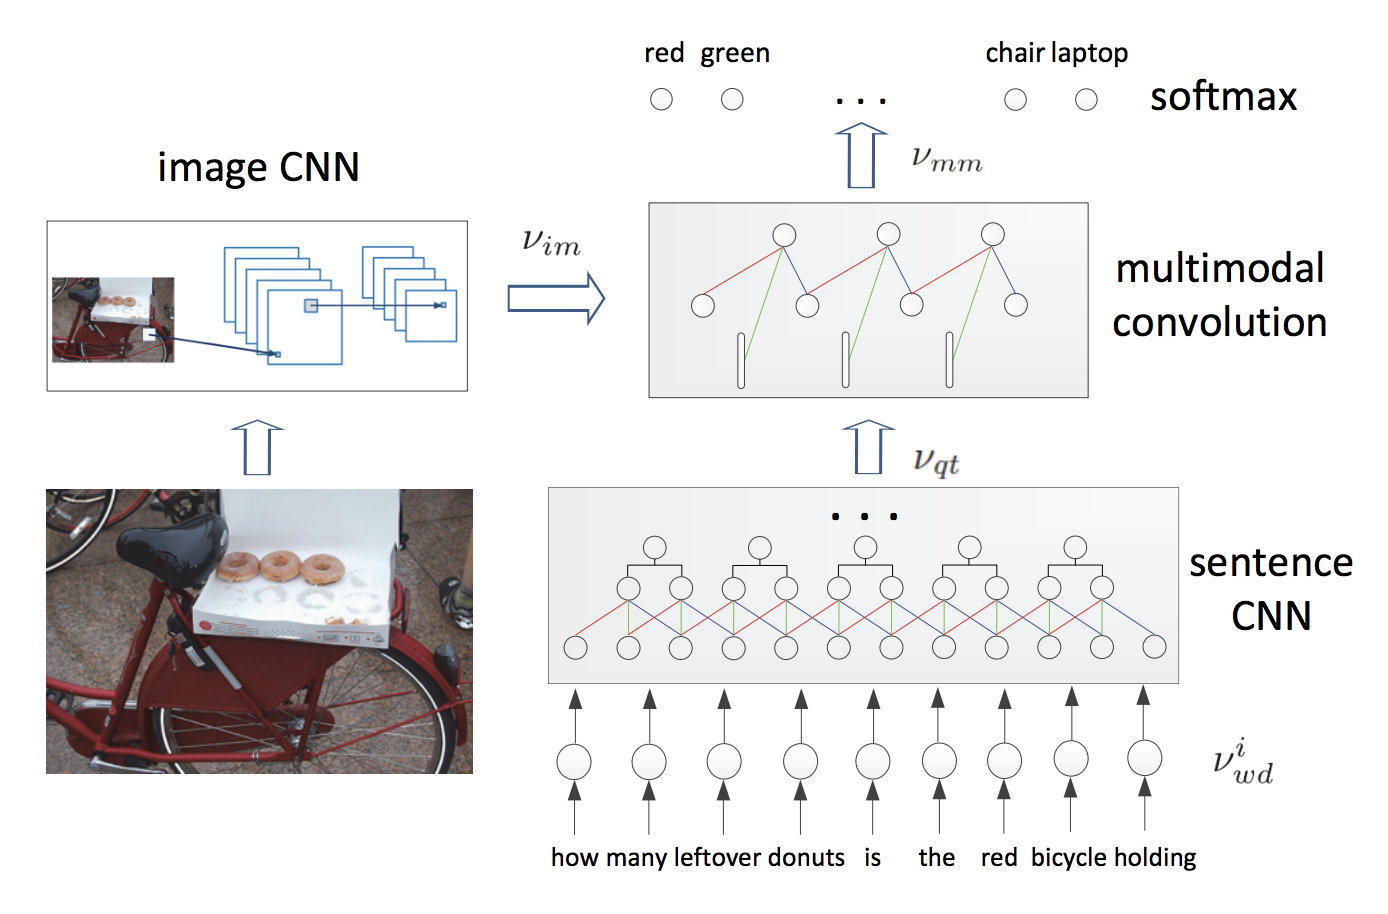
\includegraphics[width=0.8\textwidth]{lin.png}
	\caption{图像特征和问题文本特征提取时均使用CNN}
	\label{lin}
\end{figure}

除了使用不同的方法提取图像和文本特征以外,联合嵌入模型的另一个能够显著改善模型准确率的方向就是实验不用特征向量融合的池化方法。Malinowski等人通过对不同的特征向量融合方法的比较,可以看出系统的准确率与特征向量融合方法有关,不同方法之间准确率最多能相差9个百分点之多\citing{malinowski2015ask}。除了以上提到的iBOWIMG采用向量串联的方式,Lin使用向量卷积的方式外,Antol等人提出的模型使用逐元素相乘的方法融合两者\citing{antol2015vqa},Saito等人认为不同的特征融合方法各有特点,会保留或损失不同的特征,为了充分利用不同方法所保留的特征,提出了一种融合逐元素相加和逐元素相乘相结合的模型DualNet。模型同样利用了使用不同卷积神经网络CNN提取的图像特征,例如在真实场景图像采用了VGG-19\citing{simonyan2014very}、ResNet-152和ResNet-101\citing{he2016deep}。DualNet对提取出的文本特征和图像特征分别使用逐元素相加和逐元素相乘的方法得到两个不同的联合向量,再将两个的联合向量串联得到最终的合成向量,如图\ref{DualNet}。
\begin{figure}[H]
	\centering
	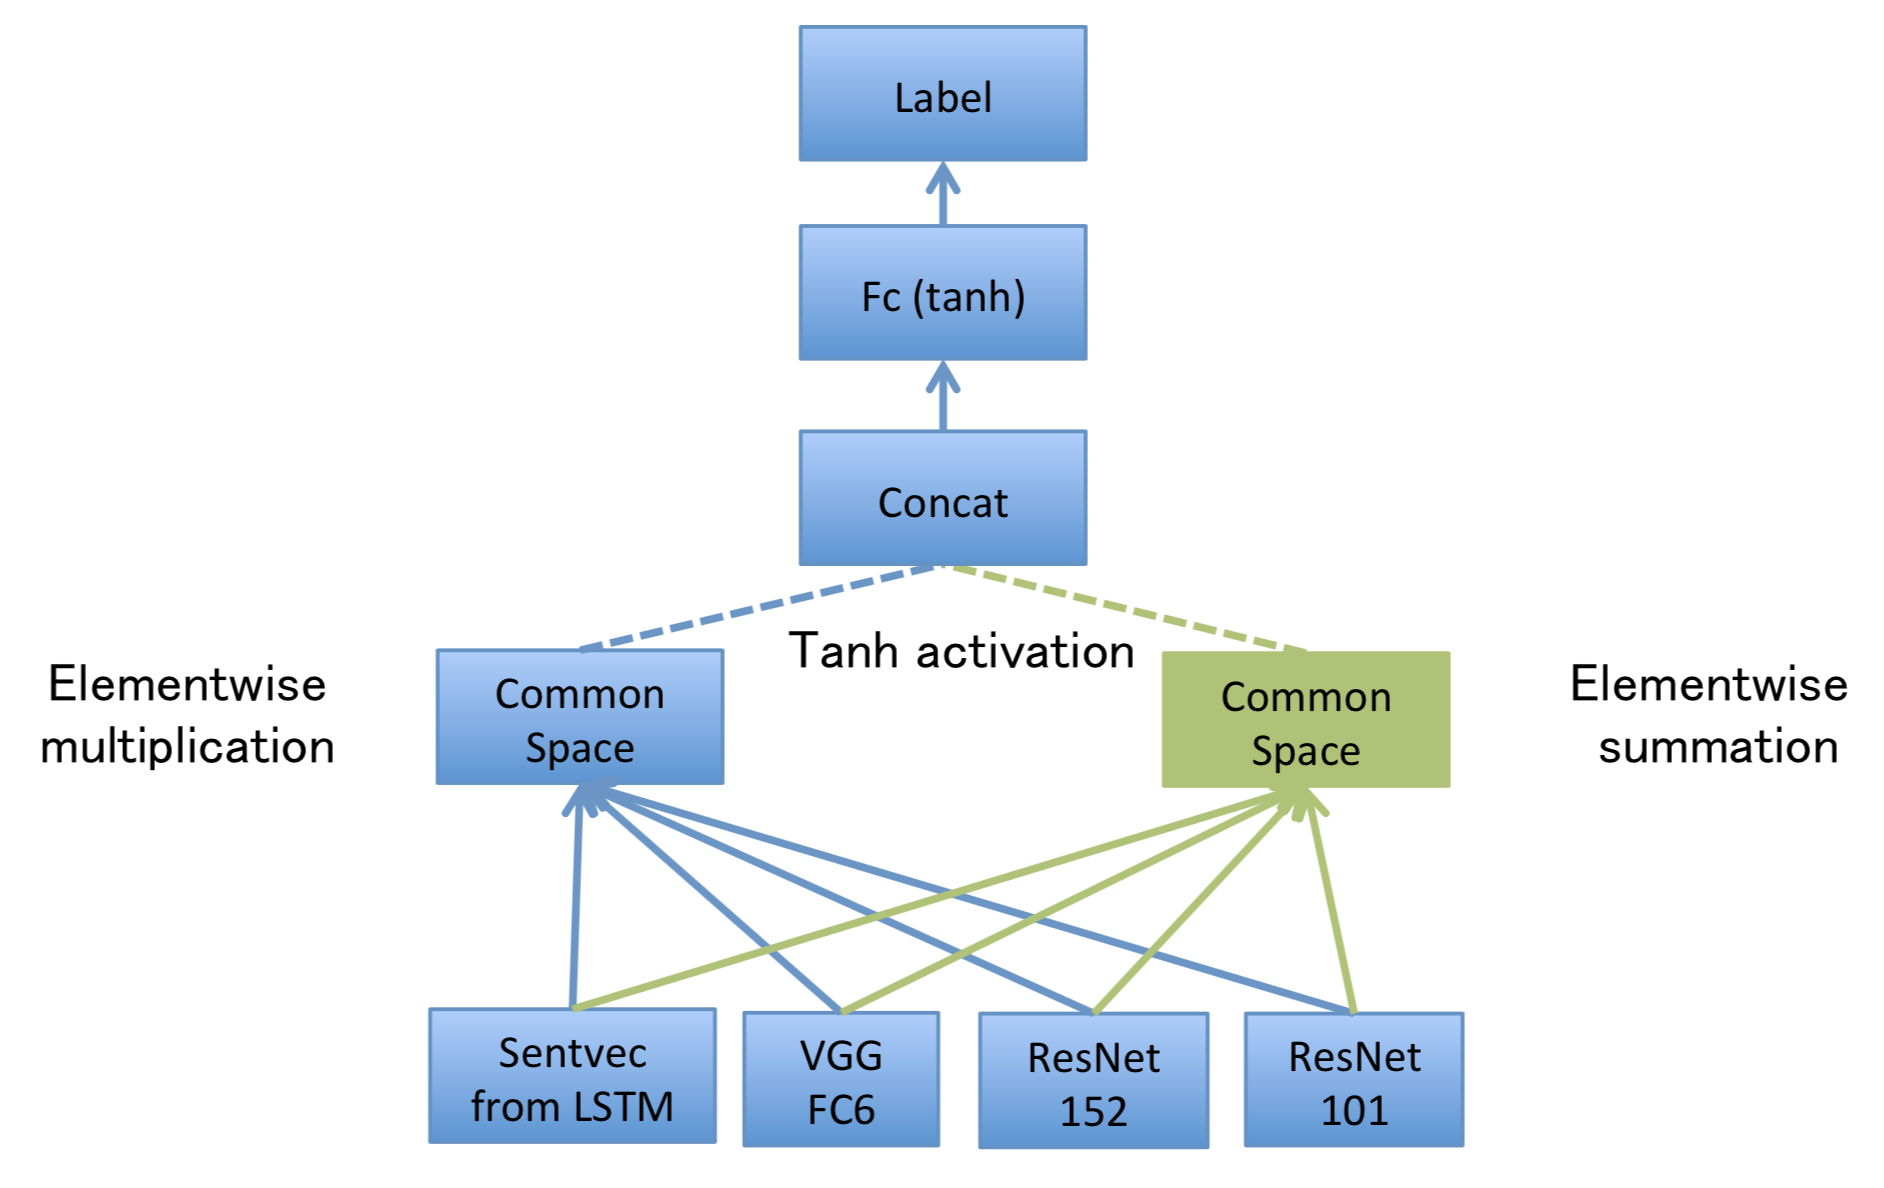
\includegraphics[width=0.8\textwidth]{DualNet.png}
	\caption{DualNet针对真实场景图像的模型架构}
	\label{DualNet}
\end{figure}

Fukui等人认为向量之间的外乘运算中,所有元素之间的互动更加活跃,应该能保留更加丰富的特征信息,因此提出一种更为复杂的多模态紧凑双线性池化方法(MCB)\citing{fukui2016multimodal}。一般的双线性模型会对两个向量的外乘结果线性化,外乘操作会得到异常高维的向量,例如外乘的两个向量维度均为2048、输出向量维度为3000时,那么训练参数的数量将达到125亿个之多,这会导致巨大的计算开销。而提出的多模态紧凑双线性方法能避免直接计算向量外乘,同时保留了大量特征,模型架构如图\ref{mcb}。
\begin{figure}[H]
	\centering
	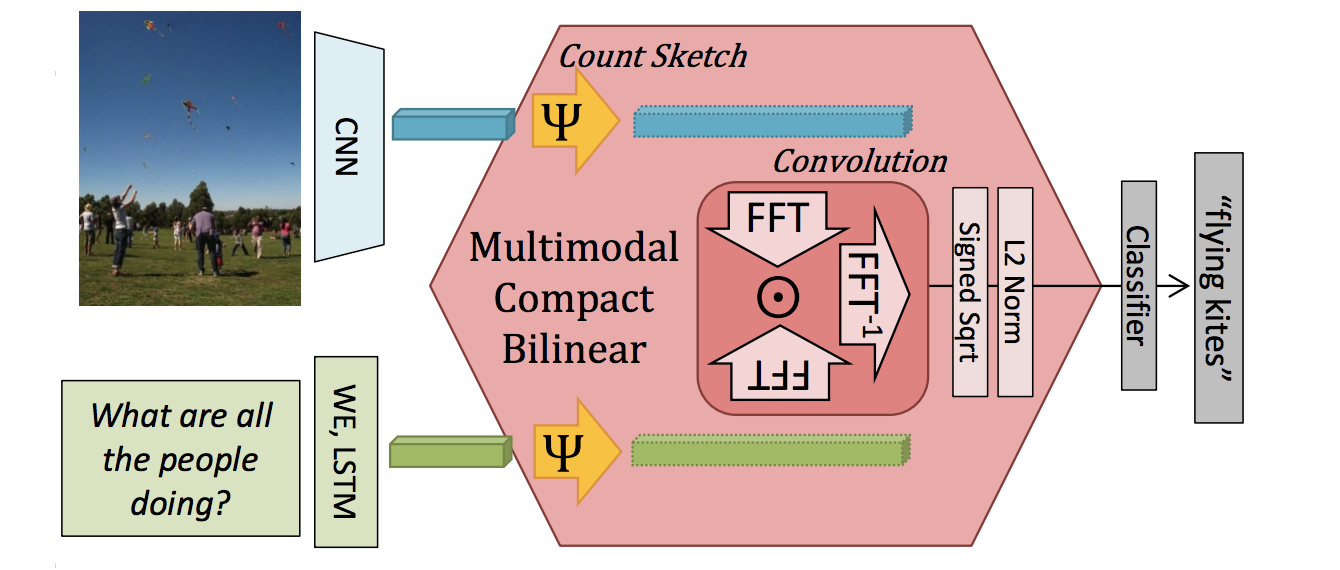
\includegraphics[width=0.8\textwidth]{mcb.png}
	\caption{使用多模态紧凑双线性池化融合图像和文本特征}
	\label{mcb}
\end{figure}

以上介绍的模型从图像特征提取、文本特征提取、特征融合方式上都做出了不同的改进和创新,但这些模型还并未引入注意力机制。由于注意力机制已经在大量的深度学习任务中表现优异,并且,近三年来的视觉问答模型大量引入注意力机制,因此,我们将带有注意力机制的模型特别提出,并加以介绍。

\subsubsection{注意力机制}
Google Deepmind团队提出了一种带有注意力机制的循环神经网络(RNN),并成功应用于图像分类任务,获得了优于以往卷积神经网络(CNN)的基线水平的分类精度\citing{mnih2014recurrent}。随后,带有注意力机制的循环神经网络便被广泛应用于自然语言处理和计算机视觉的多个子领域\citing{bahdanau2014neural, xu2015show, NIPS2015_5847}。Bahdanau等人将注意力机制引入神经机器翻译任务,仍然使用“编码-解码”的翻译模式,但一改以往将源语言文本映射为一个固定长度的向量的编码方式,而是将原语言文本编码为向量序列,解码时将翻译和位置对应因素联合学习,训练向量序列中各向量对翻译词组的不同权重,加和完成翻译结果的推断,得到了以往最优的结果\citing{bahdanau2014neural}。Xu等人受到注意力机制在机器翻译和物体识别任务成功应用的启发,将带有注意力机制的循环神经网络应用于自动生成图像标注,并且在Flickr9k, Flickr30k 和MS COCO 三个数据集上均获得了最优的结果\citing{xu2015show}。随后,更多注意力机制的变型或优化研究均在图像标注任务上展开\citing{ 7243334, wu2017global, li2017image, lu2017knowing}。

相较起图像标注任务,视觉问答任务除了要求系统能理解图片内容,生成语义和句式合理的自然语言文本以外,还需要联合学习问题文本和聚焦与问题相关的图像细节。这些任务特性决定了视觉问答任务可以利用已有较为先进的图像标注任务的框架,同时融合自然语言处理的最新成果。注意力机制在自然语言处理和计算机视觉上的成功应用便成为了视觉问答算法快速发展的基石。

Chen等人最先将注意力机制引入视觉问答任务,提出了基于注意力机制的可配置卷积神经网络(ABC-CNN)用于针对“图像问题对”生成对应的注意力映射,将问题的语义信息和图像区域建立映射,使得答案生成取决于被关注区域,减少无关区域的影响\citing{chen2015abc}(模型架构如图\ref{abc-cnn})。在Toronto COCO-QA\citing{ren2015exploring}, DAQUAR\citing{ malinowski2014multi}, 和VQA\citing{antol2015vqa}三个数据集上的测试结果都提升了最优结果,证明了注意力机制在提高视觉问答任务上的有效性,同时注意力权重图能反应系统的推理过程,为参数的微调提供了依据。
\begin{figure}[H]
	\centering
	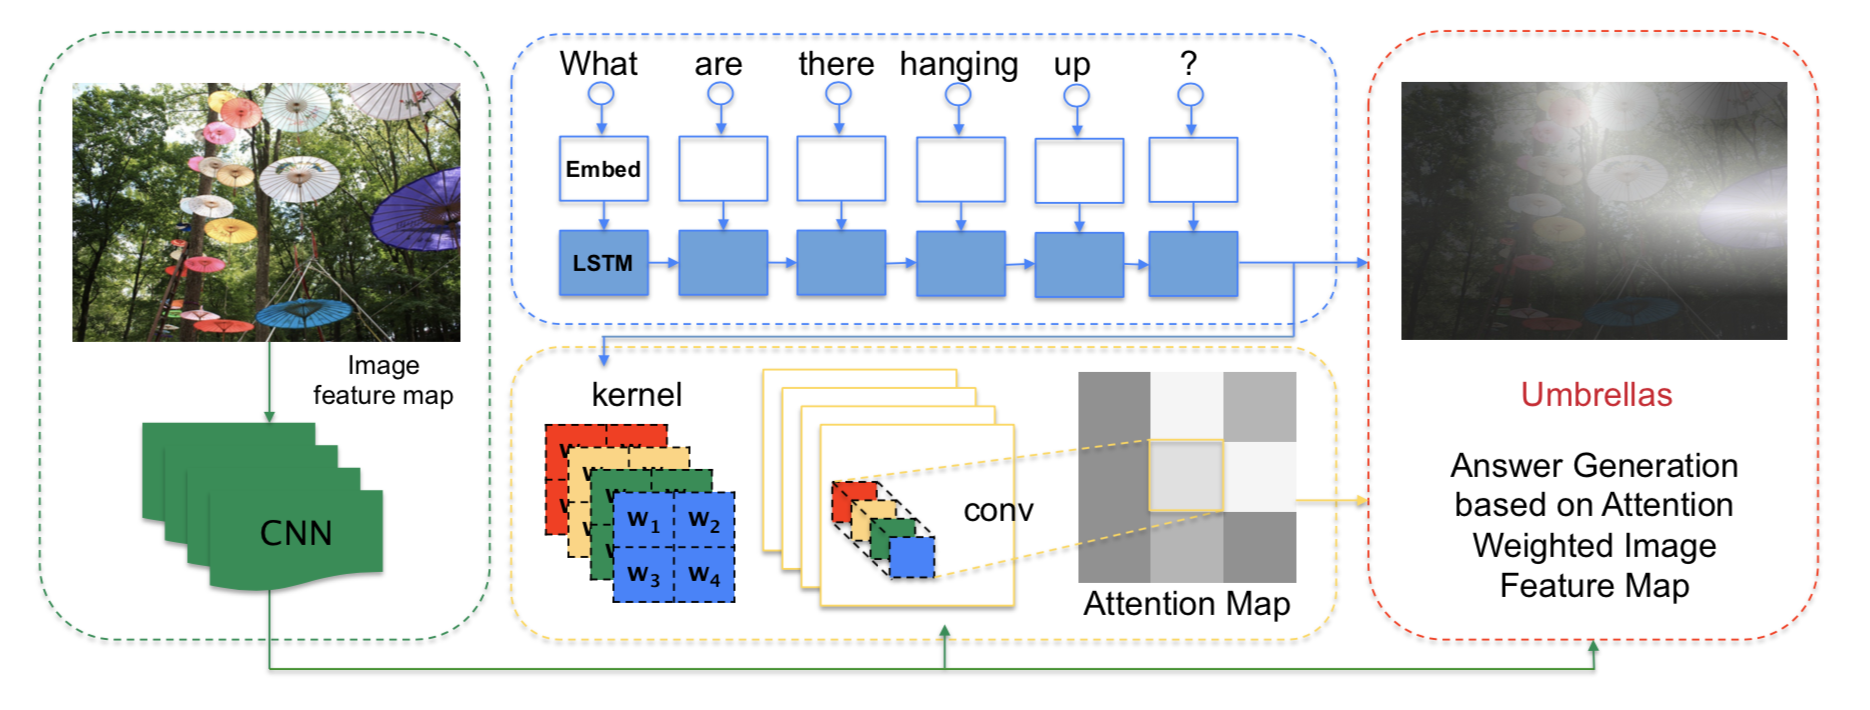
\includegraphics[width=0.8\textwidth]{abc-cnn.png}
	\caption{ABC-CNN使用CNN提取图像特征,LSTM提取问题文本特征,黄色方框内为用于推测与问题相关的图像区域的注意力机制}
	\label{abc-cnn}
\end{figure}

Shih等人使用简单的word2vec方法编码“问题-答案”对,使用预处理后的卷积神经网络CNN对图片的不同区域编码,将编码后的文本特征向量和图片特征向量映射到同一特征空间,根据特征之间的点乘运算决定每个图像区域的权重,最后结合权重化以后的图像特征和文本特征得出答案。架构如图\ref{shih}。在辨别物体颜色的任务上得到了最优结果\citing{ shih2016look}。类似的工作还有Ilievski等人提出的“聚焦型动态注意力模型“\citing{ilievski2016focused}。
\begin{figure}[H]
	\centering
	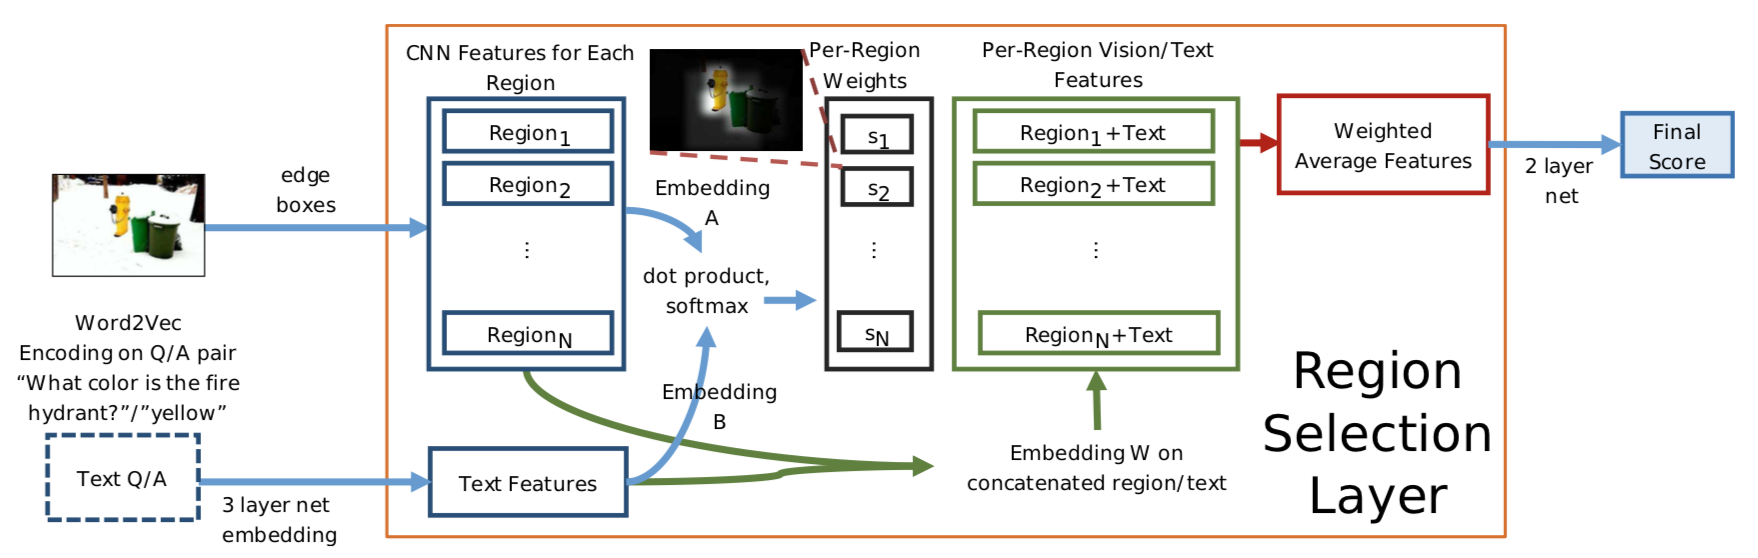
\includegraphics[width=0.8\textwidth]{shih.png}
	\caption{使用图片区域选择层实现注意力机制的架构}
	\label{shih}
\end{figure}

包括以上提到的在内,多数注意力机制对问题文本和图像区域特征进行一次运算,直接生成图像注意力权重图。针对这种情况,Yang等人提出堆栈式注意力网络——使用问题的语义表达对图像进行多次查询,不断缩小答案相关区域,实现更高的精度\citing{yang2016stacked}。注意力机制在视觉问答上的其他应用还有,同时使用对图像和问题使用注意力机制的联合注意力模型\citing{NIPS2016_6202};不采用图像区域赋值方法,而是过滤掉不相关区域的“自适应硬性注意力网络”\citing{malinowski2018learning}。

对于神经网络训练这类参数密集和计算密集的框架,注意力机制能带来两个重要的改变。一方面,无论对于图像输入还是文本输入,原有的方法都选择将输入看做一个整体,因此映射后的向量需要包含完整的输入信息,对于包含词组过多文本或是场景过于复杂的图像,编码后的向量根本无法区分开输入的局部特征,这使得神经网络的可解释性大大降低。引入注意力机制后,编码方式改变,将输入视为为局部信息的综合,保留了文本中单词和图像中像素区域的信息,通过可视化处理,能清晰的看出神经网络的推理过程,增强了系统的可解释性,可以称之为一种“弱化黑盒的处理”。另一方面,注意力机制非常符合人类对于语言和视觉信息的处理方式,这背后的假设是:针对绝大多数任务,只需要从信息源的局部便能获得充分正确的答案。类似于人类,具有注意力机制的智能体应当能获得更高的执行的效率和更高的答案精度。

\subsubsection{动态记忆网络}
无论是在自然语言理解还是图像内容理解,人类在获取单词或者图像像素区域的语义时不会将其与语境割裂来看,通常上下文语境对于准确理解文本和图像信息是非常重要的,因为在语言和图像中存在大量具有歧义特性的内容,例如,在语言中一个单词具有不同的语义,也可能有不同的词性,只有在上下文的语境中才能确定词语的真正含义。记忆力与上下文语境相似,是神经网络在训练过程中存储的“经验”,这种“经验”有助于以后的训练,这种累积经验能创造更准确的答案,基于这样的假设,研究人员为从序列化的输入中获得更准确的输入,而引入了动态记忆网络\citing{jiang2015compositional,kumar2016ask,xiong2016dynamic}。

Jiang等人在常见的CNN解析图像、LSTM解析问题文本的架构上,新增一个成分记忆模块\citing{jiang2015compositional},旨在融合每一次训练过程中的局部图像信息和文本信息,并提供给下一次训练使用,从而使网络存储了训练过程的“经验”,这与之后提出的动态记忆网络有同样的思想,模型训练流程如图\ref{c-memory}。
\begin{figure}[H]
	\centering
	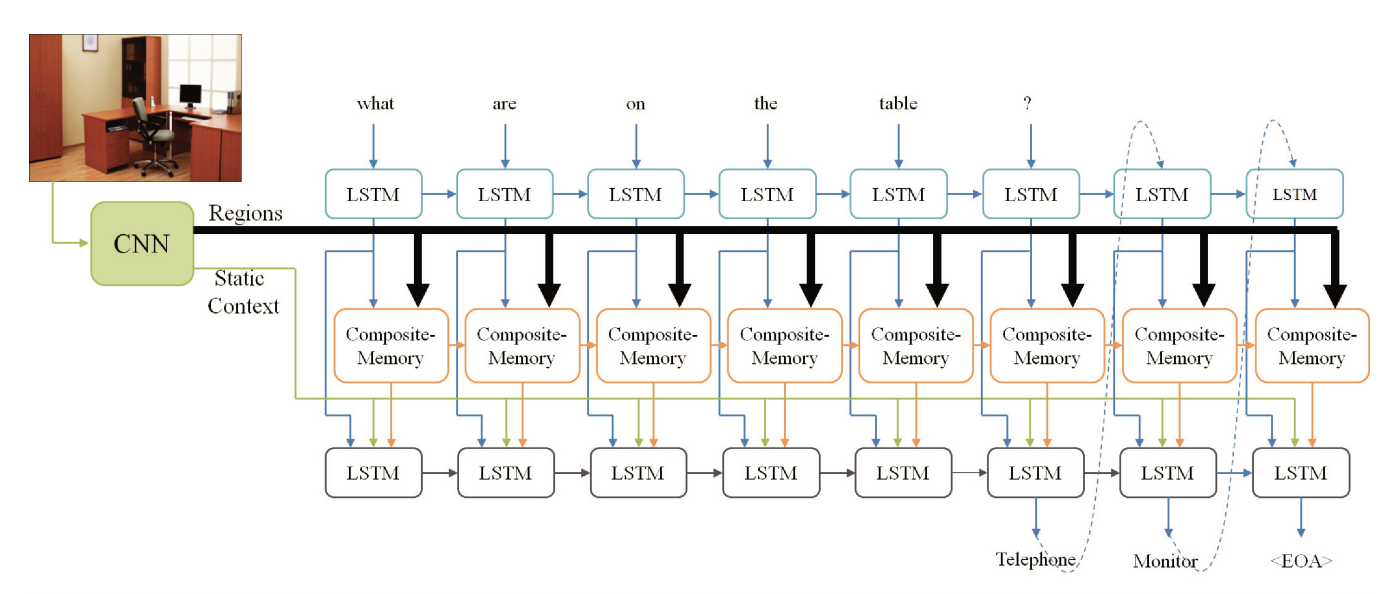
\includegraphics[width=0.8\textwidth]{c-memory.png}
	\caption{成分记忆模型的训练流程}
	\label{c-memory}
\end{figure}

Kumar等人为解决文本问答(Text-QA)任务而提出动态记忆网络(DMN)\citing{kumar2016ask}。动态记忆网络(DMN)是一个用于生成文本问题答案的神经网络框架,它由输入模块、问题模块、情节记忆模块和问题模块构成,输入模块用于编码文本输入;问题模块用于编码文本问题;情节记忆模块接受由输入和问题模块得到的分布式向量,再使用注意力机制选择部分接受到的向量,结合选择后的向量与以往存储的“记忆”生成新的“记忆”向量,并不断迭代;答案模块根据最终的记忆向量生成答案,模型架构如图\ref{dmn}。
\begin{figure}[H]
	\centering
	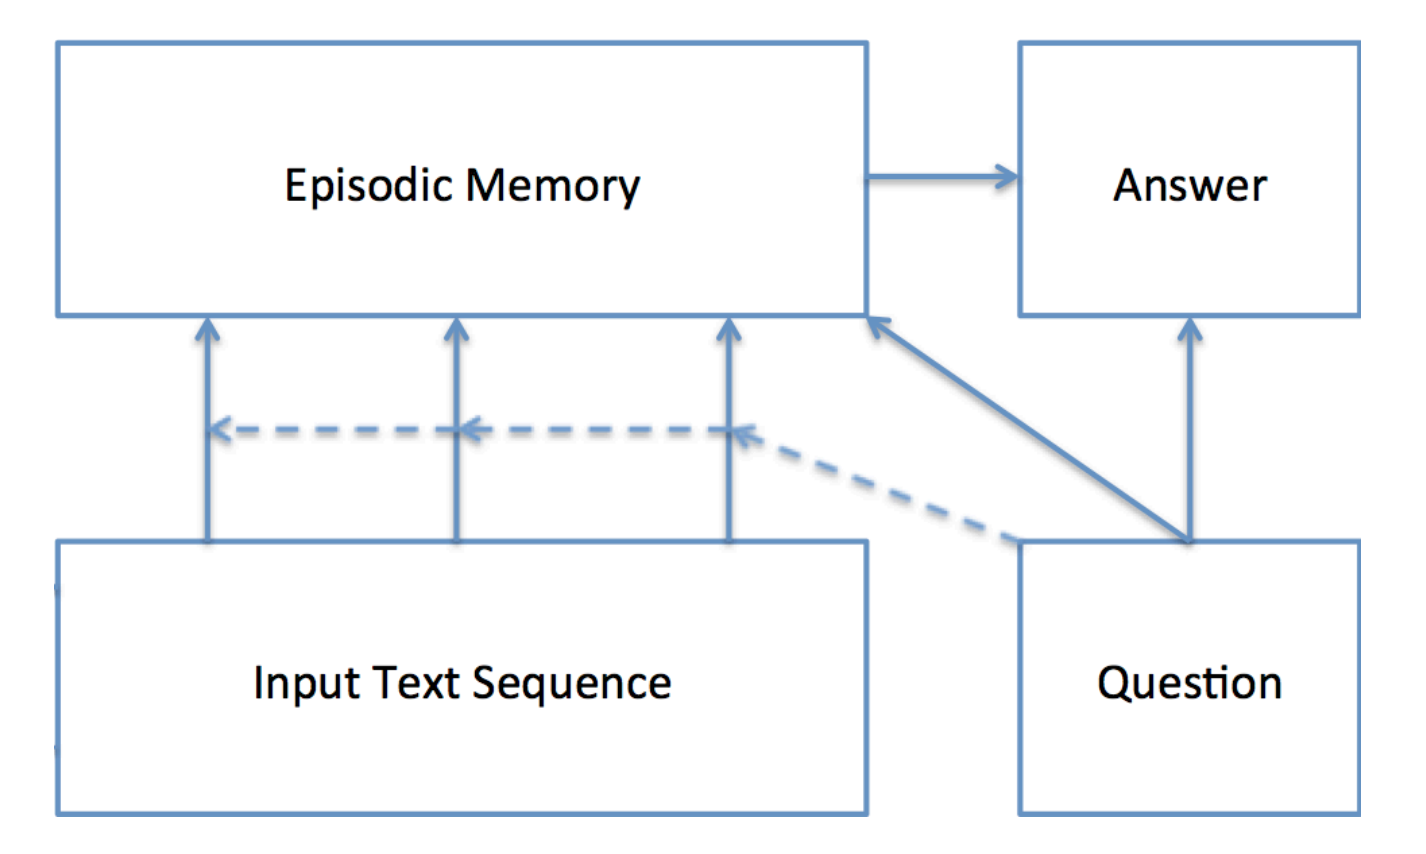
\includegraphics[width=0.5\textwidth]{dmn.png}
	\caption{DMN基础架构}
	\label{dmn}
\end{figure}

动态记忆网络(DMN)在文本问答、语义分析、词性标注任务上取得了最优的结果,受到其在处理序列化的文本信息上的优异表现的启发,Xiong等人在原有网络的基础上改善了输入和记忆模块,除了能处理文本信息外,还能处理图像信息,提出应用到于视觉问答任务动态记忆网络+(DMN+)\citing{xiong2016dynamic},如图\ref{v-dmn}。动态记忆网络+(DMN+)将原有的输入模块中处理文本编码的门控复发单元(GRU)更换为双向门控复发单元(bi-GRU)以得到文本或图像区域更完整的上下文信息;使用基于注意力机制的门控复发单元替换原有的软性注意力机制。更新后的动态记忆网络+(DMN+)在DAQUAR\citing{malinowski2014multi}和VQA数据集\citing{antol2015vqa}上的测试结果都得到了具有竞争力的表现。
\begin{figure}[H]
	\centering
	\subfigure[应用于文本问答的动态记忆网络(DMN)模型架构]{
		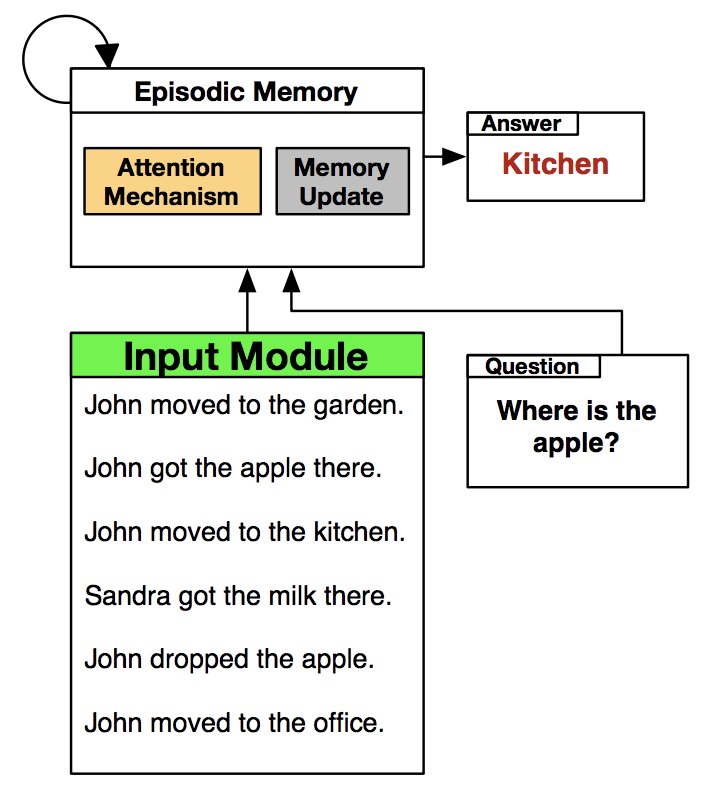
\includegraphics[width=0.4\textwidth]{t-dmn.png}}
	\subfigure[应用于视觉问答的动态记忆网络+(DMN+)模型架构]{
		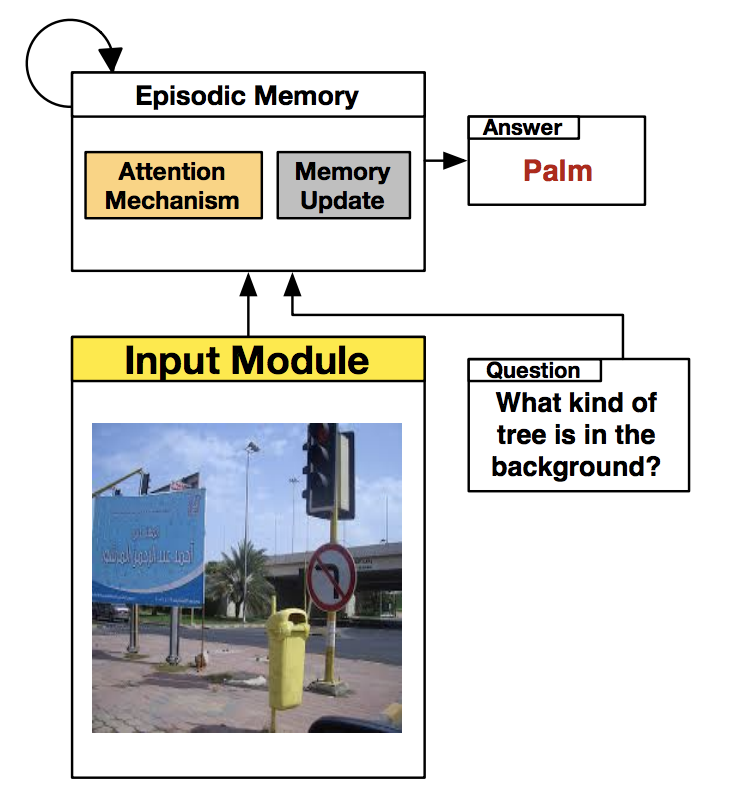
\includegraphics[width=0.4\textwidth]{v-dmn.png}}
	\caption{DMN+与DMN架构对比}
	\label{v-dmn}
\end{figure}

\subsection{基于外源知识库的视觉问答模型}
视觉问答任务基于图像场景回答问题,图像理解、问题理解和答案生成是实现准确的视觉问答系统的算法核心。图像理解、问题理解和答案生成三者又可以根据人类思考逻辑将其划分为两个逻辑层次,问题理解成为逻辑基点,图像理解和答案生成都根据问题的不同而采用适当的算法策略——注意力机制便是一种借助问题理解而实现计算效率更高的图像解析方法,答案生成中关心的答案类型和答案词组长度也需要依照问题的不同而选择。因此问题的解析过程对于视觉问答算法的准确性和计算成本都有很大的影响。

正如上文提及的,问题可以分为识别和推理两个大类,推理任务中既要求系统能准确识别图像中的对象,往往也会涉及图像中无法获取的先验知识。先验知识包括众所周知但不会显性呈现的常识和面对特定领域需要具备的专业知识,例如,判断路口是否可以通行时,涉及基本交通规则的常识,判断艺术品的作者这类专业问题时,需要借助与该艺术品相关的知识储备。

先验知识对视觉问答系统提出了更高的要求,这也揭露了主流的联合嵌入模型的缺陷:

第一,数据集依赖。联合嵌入模型的答案生成来源于训练集中的问题和答案文本,这意味着训练集中包含的知识和文本内容是整个视觉问答系统的所有知识来源,因此对于测试集中涉及的全新概念或答案,系统根本无法得出正确的答案。不断扩充包含更多先验知识的训练集是提高精度的方式之一,但对于整个世界蕴含的不可计量的知识而言,这种数据集扩充的方式成本巨大。

第二,网络容量小。联合嵌入模型要求网络本身能存储学习到的知识,目前网络的容量相较于需要学习的知识是严重不足的。

第三,黑盒效应明显。对于识别和分类等问题而言,可解释性与高精确度相比,显得不那么重要,但是对于需要明确推理过程的问答系统而言,黑盒的不可解释性会降低提问者对系统的可信度。

对于以上三个联合嵌入模型的缺陷,一种可行的解决方案是将推理过程和知识学习分离,引入外源知识库。可扩展的外源知识库可以解决网络容量的限制问题;知识库中结构化的数据能为推理提供路径,提高系统的可解释性。因此基于知识库的视觉问答模型是并行于联合嵌入模型的另一个重要研究方向。

在基于知识库的视觉问答模型中,知识库的使用方式分为两类。一类为知识库查询类,依照查询知识库查询获得答案的思路,模型提取图片的实体、将实体映射到知识库、转化自然语言为查询语句、查询知识库。代表模型为Ahab\citing{wang2015explicit}和FVQA模型\citing{wang2017fvqa}。这些模型依靠精准的查询语句,对于预先设定好的模板问题能实现优于基线模型的准确率,然而却面临着问题模板设计成本高、数据集难构建、模型泛化能力差等缺点。

另一类为知识库嵌入类,这种方式不用设计复杂的查询语句,而是将知识库的数据转化为额外的特征向量,并联合图像特征和问题特征一起训练。这种方式能省去问题模板和查询语句设计的人工成本,并将模型在更大规模的开放性数据集进行训练。代表为基于知识库的通用嵌入模型\citing{wu2016ask}。

本节将简单介绍以上两类基于知识库的模型,并指出其优缺点。

\subsubsection{知识库查询类}

\textbf{Ahab}
Wang等人提出的Ahab视觉问答系统利用DBpedia作为知识库,实现对需要先验知识的问题的推理应答,即使问题中涉及不包含于图像中的概念\citing{wang2015explicit}。Ahab的主要思路为三步,第一步,将图像中的概念链接到知识库中相同的概念,形成从图像到知识库的映射,第二步,将自然语言的文本问题处理为知识库查询语句,实现从自然语言的句法和语义结构变换到相应的查询语句结构,第三步,将知识库的查询结果转换为自然语言表达。利用以上三步,Ahab可以不通过数据集训练获取知识,而使用自然语言到知识库的两次转化完成问答任务。

具体来说,为了建立图像概念到知识库实体之间的映射,首先检测图像包含的概念,再将提取出的图像概念和知识库实体建立链接。Ahab分别使用预训练的Fast R-CNN\citing{ren2015faster}和两个不同的VGGnet\citing{simonyan2014very}从图像中提取物体对象、图像场景和图像属性三种视觉概念。所有提取出的图像信息都使用资源描述框架(RDF)的形式表示,例如,“图像中包含长颈鹿对象”被表示为(图像,包含,对象1),(对象1,名称,长颈鹿)。每个视觉概念则被直接链接到具有相同语义的知识库概念,如图所示\ref{linkingMathord}。
\begin{figure}[H]
	\centering
	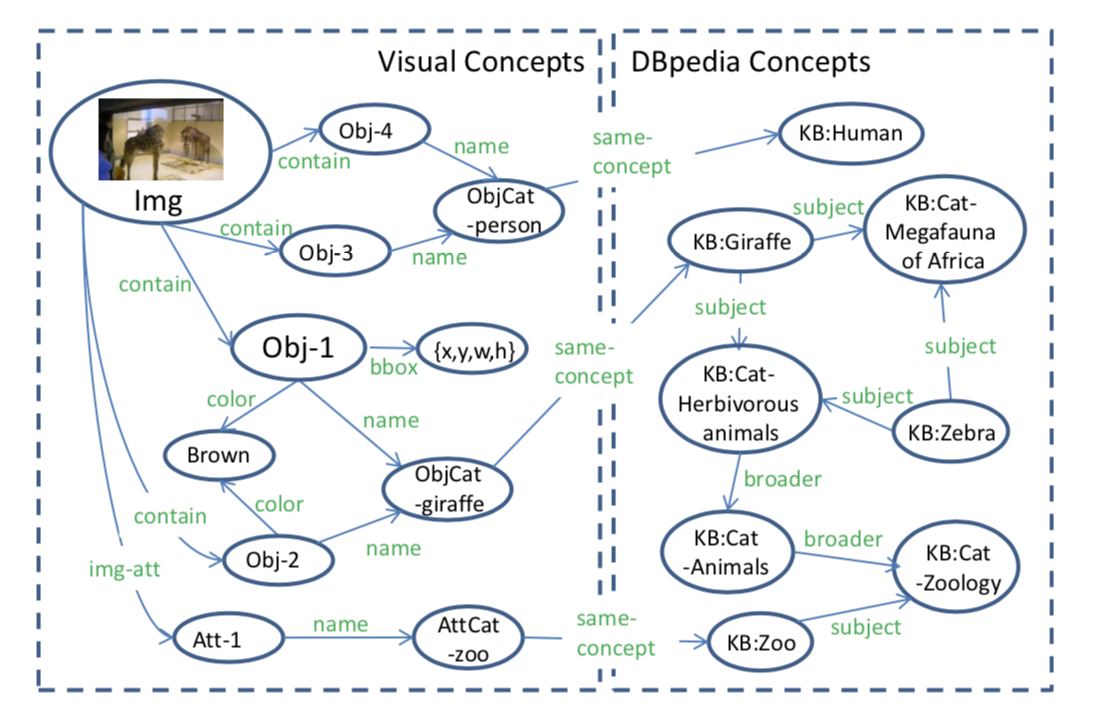
\includegraphics[width=0.8\textwidth]{linkingMathord.png}
	\caption{Ahab中链接图像信息和知识库实体的RDF图结构}
	\label{linkingMathord}
\end{figure}

在问题文本处理方面,Wang等基于自建的KB-VQA数据集——其中的问题需要常识或外源知识,设定了23种问题模板,将自然语言问题转化为相应的知识库查询语句,直接从知识库中查询得到答案。Ahab在KB-VQA数据集上的表现如图\ref{ahab_evaluation}。
\begin{figure}[H]
	\centering
	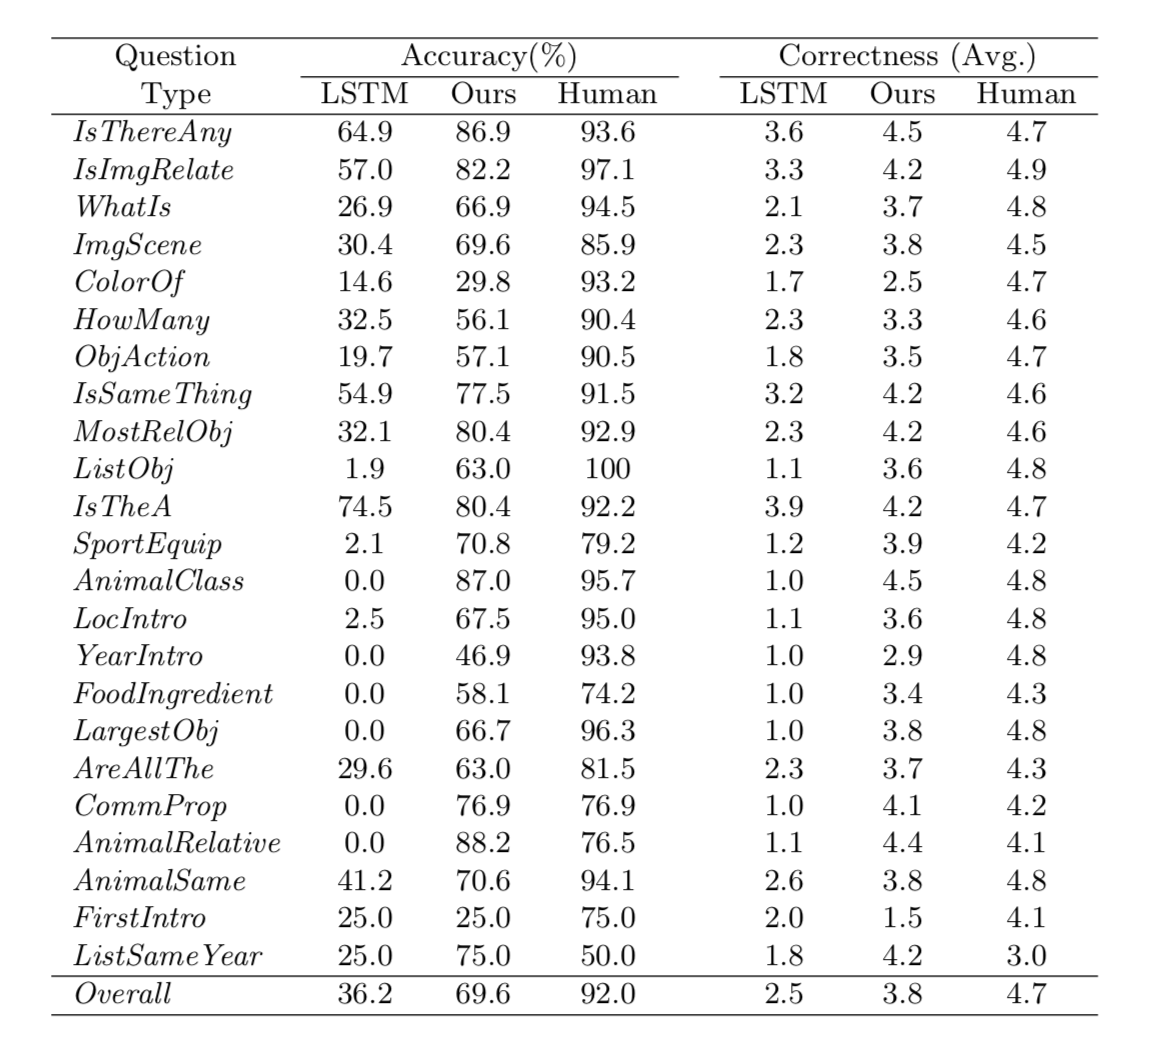
\includegraphics[width=0.8\textwidth]{ahab_evaluation.png}
	\caption{Ahab、联合嵌入模型和人类作答在23种问题上的表现。Accuracy是得分超过3的问题数量的比例,Correctness是某类问题得分的加权平均数。}
	\label{ahab_evaluation}
\end{figure}

从图\ref{qtd}中可以看出,Ahab在每种问题类型上都优于联合嵌入模型,但离人类的正确率还是有一定差距,尤其在“判断物体颜色”和“比较两个物品的诞生先后”两种问题。但是由于KB-VQA在不同问题类型上数量的不均衡和问题样本数过小的缺陷,Ahab在真实场景中对于推理问题的解决上仍然有待检验。

Ahab模型最大的缺点是,模型的准确率高度依赖问题模板和查询语句的人为设计。人为设计必将带来的高额成本,并且需要使用特定的数据集进行训练。当问题类型数量剧增时,人工的对每种类型设定对应的算法是不切实际的,因此Ahab的扩展性面临挑战。

但相较于主流使用统计方法的联合嵌入模型,Ahab利用知识库取代知识学习过程的方法在复杂推理任务,尤其是需要运用先验知识的问题上,表现更好。

\textbf{FVQA}
Ahab将问题解析为知识库查询语句时,需要预先确定问题模板,这极大的限制了系统面对多样化问题的能力,因此Wang等人改变了问题到查询语句的映射方式提出了FVQA模型\citing{wang2017fvqa}。FVQA模型使用长短期记忆(LSTM)网络训练一个28类的查询语句分类器,实现将问题到查询语句的分类过程。通过LSTM的分类,文本问题被映射为(REL, AS, VC)的查询类型,其中VC表示视觉概念、REL表示谓语、AS表示知识来源。对于所有28种查询类型,查询语句都由下面的形式构成:
\begin{verbatim}
Find ?X, ?Y, subject to 
	{(ImgID,Contain,?X) and (?X,VC-Type,VC) and (?X,REL,?Y)}
\end{verbatim}
其中ImgID表示图片的标号,?X表示在图片ImgID中类型为VC的视觉概念,?Y表示在知识库中与?X通过谓语REL链接的概念。再根据AS是图片还是知识库的类型,使用不同的方法得到最终的答案。

引入支持向量机(SVM)\citing{chang2011libsvm}和使用长短期记忆(LSTM)的联合嵌入模型\citing{wu2016value}作为基线模型:只提供问题的SVM-Question和LSTM-Question、只提供图片的SVM-Image和LSTM-Image以及同时提供问题文本和图片的SVM-Question+Image和LSTM-Question+Image,各模型使用自建的FVQA数据集作为训练和测试集中测试,不同模型的正确率见表\ref{fvqa_table}。
% Please add the following required packages to your document preamble:
% \usepackage{multirow}
% \usepackage[table,xcdraw]{xcolor}
% \usepackage{booktabs}
% If you use beamer only pass "xcolor=table" option, i.e. \documentclass[xcolor=table]{beamer}
\begin{table}[H]
% \resizebox{0.5\textwidth}{!}{}
\caption{不同模型在FVQA数据集上的测试正确率,Top-1表示只取得分最高的预测结果,Top-3和Top-10以此类推。灰色数据表示使用与问题对应的完全正确的查询类型时的正确率。}
\begin{tabular}{lccc}
\toprule
\multicolumn{1}{c}{} & \multicolumn{3}{c}{Overall Acc. (\%)}\\
\cmidrule(r){2-4}
\multicolumn{1}{c}{\multirow{-2}{*}{\textbf{Method}}} & \textbf{Top-1}& \textbf{Top-3} & \textbf{Top-10} \\
\midrule
SVM-Qusetion        & 11.19 & 20.68 & 32.14 \\
SVM-Image           & 17.55 & 30.75 & 49.02 \\
SVM-Qusetion+Image  & 17.99 & 31.83 & 49.55 \\
LSTM-Question       & 10.30 & 18.26 & 31.02 \\
LSTM-Image          & 22.69 & 36.21 & 58.59 \\
LSTM-Question+Image & 23.37 & 37.02 & 52.51 \\
\midrule
\cellcolor[HTML]{C0C0C0}gt-QQmaping & \cellcolor[HTML]{C0C0C0}64.23 & \cellcolor[HTML]{C0C0C0}71.58 & \cellcolor[HTML]{C0C0C0}72.74 \\
top-1-gt-QQmaping & 53.63 & 60.70 & 61.59 \\ 
top-3-gt-QQmaping & \textbf{58.19} & \textbf{65.89} & \textbf{66.83} \\
\bottomrule
\end{tabular}
\label{fvqa_table} 
\end{table}

从表\ref{fvqa_table}中Top-1一列可以看出,无论是SVM-Question+Image与SVM-Image之间的正确率差距还是LSTM-Question+Image与LSTM-Image的正确率差值都非常小,这说明问题的解析对于SVM和LSTM这两种模型正确率的提升没有太大的帮助,而两个模型总体的正确率也处于较低的水平,说明统计方法在样本较小的语料库中很难学习到知识间真正的逻辑关联。而FVQA模型使用问题到查询映射模型能从问题文本中提取到关键信息,并能利用关键信息组成有意义的语言结构,再结合额外知识库搜索到正确答案,答案获得的过程反映了推理的过程。gt-QQmaping(灰色背景)使用问题对应的正确查询类型,因此正确率反映了理想状况下FVQA模型从查询类型到生成查询语句过程中的误差情况,知识库查询过程的错误率在30\%左右。top-1-gt-QQmaping与gt-QQmaping之间的差距则代表问题到查询类型的正确率在最终答案的影响,top-3-gt-QQmaping的准确率高于top-1-gt-QQmaping的原因在是因为前者拥有更高的问题到查询类型映射的准确率。

表\ref{fvqa_answerSource}提供了不同方法在不同答案来源上的正确率,对比表中Image和KB两列容易看出,答案来源于视觉概念的准确率在所有模型上均远高于知识库来源,这说明表中涉及的三种模型都只能从图像和问题文本中包含的概念中提取答案,一旦答案涉及都额外知识库中的“新”概念,准确率便急剧下降,即使是使用额外知识库的gt-QQmaping。
\begin{table}[H]
% \resizebox{0.8\textwidth}{!}{}
\centering
\caption{不同方法在不同答案来源上的正确率}
\begin{tabular}{lcccccc}
\toprule
\multicolumn{1}{c}{\multirow{3}{*}{\textbf{Method}}} & \multicolumn{6}{c}{Answer-Source}\\
\cmidrule(r){2-7}
 & \multicolumn{3}{c}{\textbf{Image}} & \multicolumn{3}{c}{\textbf{KB}}\\
\cmidrule(r){2-4}
\cmidrule(r){5-7}
 & \textbf{Top-1} & \textbf{Top-3} & \textbf{Top-10} & \textbf{Top-1} & \textbf{Top-3} & \textbf{Top-10} \\
 \midrule
SVM-Qusetion        & 12.80 & 24.53 & 36.48 & 0.68 & 2.03 & 3.72 \\
SVM-Image           & 19.92 & 34.88 & 55.11 & 2.03 & 3.72 & 9.12 \\
SVM-Qusetion+Image  & 20.43 & 36.07 & 55.73 & 2.03 & 4.05 & 9.12 \\
LSTM-Question       & 11.71 & 20.49 & 34.21 & 1.01 & 3.72 & 10.14 \\
LSTM-Image          & 25.49 & 40.40 & 65.12 & 4.39 & 8.78 & 15.88 \\
LSTM-Question+Image & 26.01 & 41.12 & 58.05 & 6.08 & 10.14 & 16.22 \\
\midrule
\cellcolor[HTML]{C0C0C0}gt-QQmaping & \cellcolor[HTML]{C0C0C0}72.65 & \cellcolor[HTML]{C0C0C0}80.13 & \cellcolor[HTML]{C0C0C0}80.13  & \cellcolor[HTML]{C0C0C0}9.12 & \cellcolor[HTML]{C0C0C0}15.54 & \cellcolor[HTML]{C0C0C0}24.32 \\
top-1-gt-QQmaping & 60.89 & 68.27 & 68.27 & 6.08 & 11.15 & 17.91 \\ 
top-3-gt-QQmaping & \textbf{66.10} & \textbf{74.15} & \textbf{74.15} & \textbf{6.42} & \textbf{11.82} & \textbf{18.92} \\
\bottomrule
\end{tabular}
\label{fvqa_answerSource}
\end{table}

FVQA模型提出了一种以句法结构中的谓语为核心的先验知识问题的解答思路,首先从问题中解析出关键的谓语信息,在问题到查询类型模型中,结合谓语、视觉概念和答案来源决定了28种不同的查询类型,再使用生成的查询语句搜索基于12种谓语构建的知识库,最终预测答案。“主语-谓语-宾语”的一般句式结构中谓语表示了主语和宾语之间的相互作用,即使在相同的主语和宾语情况下,不同的谓语能表达出截然不同的语义信息,而绝大多数问题也能够直接通过谓语,推断答案的范畴。以谓语为基础的优势有几点,第一,易于问题分类。问题的自然语言表达方式众多,但无论如何改变句式结构,表达相同含义的谓语有限,通过对谓语的语义划分能够划分出问题的不同类型。第二,便于知识库的查询。知识库中的实体之间通过不同的谓语连接,形成错综复杂的知识网络,一个实体有众多连接,但一个谓语只连接两个实体,且往往谓语的两端就是问题的答案。

FVQA模型的缺陷有三点,第一,分类数量的确定和分类模型的精度。FVQA模型由于查询语句的生成依赖于查询类型,因此问题到查询类型映射的准确性会直接影响到答案生成的正确率。表\ref{fvqa_table}是在FVQA数据集上进行的,由于数据集中问题的类型只有28种,因此FVQA模型在问题到查询类型映射模型中使用了28类的分类器,但在实际问答环境中问题类型的具体数量远远多于28种,且无法预先确定。想训练能应用于实际情景中,FVQA模型不仅需要数据集的扩充,还需要提高模型本身的分类精度。第二,不能回答以谓语为答案的问题。所有28种查询类型都要求能从问题中提取关键谓语,并且所有答案都是物体对象,如果问题询问对象之间的关系,模型则无法从问题文本中获得谓语,不能得到答案。第三,不能很好的处理含有多个动词的复杂推理问题。FVQA模型的查询语句过于简单,仅仅将一次查询结果作为答案,在面对需要多级推理的问题时,便无法直接得到答案。

\subsubsection{知识库嵌入类}

知识库查询类模型通过将问题转换为特定的知识库查询语句,限制了问题类型。为了提高视觉问答系统的问题的灵活性,Wu等人又通过改进常见的CNN+LSTM的嵌入模型,提出了基于知识库的通用嵌入模型\citing{wu2016ask}。模型的基本架构由图像属性提取网络(CNN)、图像描述生成网络、外部知识库查询网络以及答案生成网络(LSTM)构成,模型架构如图\ref{KBLSTM}。
\begin{figure}[H]
	\centering
	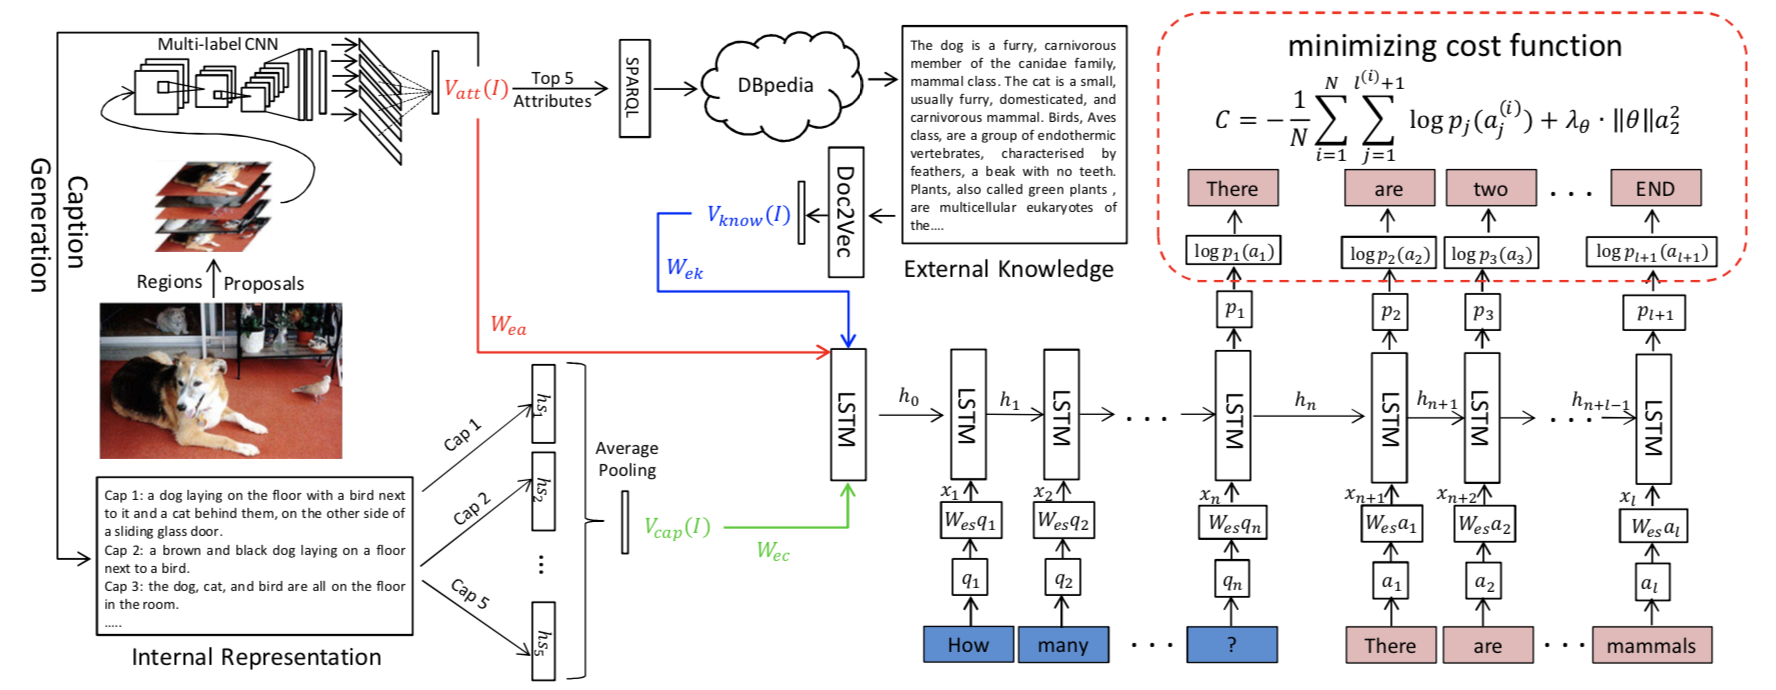
\includegraphics[width=0.8\textwidth]{KBLSTM.png}
	\caption{结合外部知识库的通用嵌入模型}
	\label{KBLSTM}
\end{figure}

图像属性提取网络将图像属性提取问题视为多标签的分类问题,以图像的多个子区域作为输入,输出前五个从MS COCO中筛选得到的图像属性$V_{att}(I)$,属性可能为物体名称、动作或者描述特征的形容词。提取出的图像属性分别作为图像描述生成网络和外部知识库查询网络的输入,图像描述生成网络将\cite{wu2016value}中的高层次的属性表达输入LSTM网络生成基于图像属性的描述,再将文本描述转化特征向量$V_{cap}(I)$。外部知识库查询网络首先分别将五个图像属性转化为知识库查询语句,查询到DBpedia知识库中相应的对象后,返回其“comment”——“comment”往往包含关于知识库对象最重要的解释信息,如图\ref{SPAQLexample}。Wu等人使用Doc2Vec\citing{le2014distributed}将其转化为$V_{know}(I)$。最后将$V_{att}(I)$、$V_{cap}(I)$、$V_{know}(I)$以及问题文本作为答案生成网络(LSTM)的输入,训练网络生成答案。
\begin{figure}[H]
	\centering
	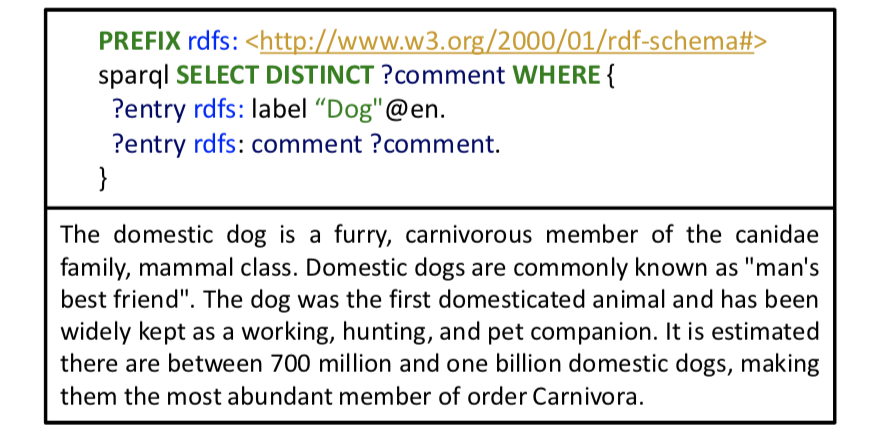
\includegraphics[width=0.5\textwidth]{SPAQLexample.png}
	\caption{使用‘dog’属性的查询语句以及返回的‘comment’内容}
	\label{SPAQLexample}
\end{figure}

在评估模型准确率时,由于该模型面对开放性问题,因此不同于Ahab和FVQA只能使用专门设计的数据集,该模型采用Toronto COCO-QA\citing{ren2015exploring}和VQA\citing{antol2015vqa}两个数据集进行评测,分别获得了69.73\%和55.96\%的准确率。

相对于知识库查询类的模型,知识库嵌入类的模型无需设计查询语句和构建数据集,因此可以使用通用数据集训练和评价;相对于不引入知识库的联合嵌入模型,基于知识库的模型能提供图像和问题以外的信息,并且具有很高的知识存储容量。

知识库嵌入类的模型的缺点是,由于答案的生成依然依赖于训练集,因此在面对复杂的推理问题时,表现差于知识库查询类的模型。

总结上文提到的所有视觉问答模型,可以看出联合嵌入模型是主流,注意力机制和动态记忆网络的出现也都是为了弥补原有联合陷入模型的计算效率不高、记忆短缺等问题。虽然引入外源知识库能更为彻底的解决神经网络知识存储不足的问题,实现特征提取和答案推理的分离,但是其下属的两个类型:知识库查询类和知识库嵌入类在多个方面仍然存在优劣。三种模型的比较可以简单描述为以下关系:
\begin{description}[labelindent=2em, leftmargin=6em, style=sameline]
\item [解决识别类问题:]知识库嵌入类>联合嵌入模型>知识库查询类
\item [解决推理类问题:]知识库查询类>知识库嵌入类>联合嵌入模型
\item [模型迁移能力:]知识库嵌入类=知识库查询类>联合嵌入模型
\end{description}

联合嵌入模型由于其模块组合的灵活性,因此具有很高的改进空间。而知识库潜入类的模型由于引入了知识库,能引入额外的特征,因此提高了其对推理问题的解决能力,有很好的研究前景,并且能够使用通用数据集训练,可实现端对端的训练。而知识库查询类的模型基于人为设计的查询模板,在推理问题上能实现更好的精度,但是查询模板和数据集的构建成本过高,限制了其进一步的发展。

\section{本文的主要贡献与创新}
虽然视觉问答任务具有广阔的应用前景和有价值的研究意义,但其仍然属于起步阶段,面临着诸多亟待解决的问题。我们认为现有的模型还存在以下三个主要问题。

第一,泛化能力受限于数据集。目前的视觉问答主流模型为联合嵌入模型,其主要思路为联合图像处理模型输出的图像特征和自然语言处理输出的文本特征,并利用神经网络训练联合后的特征,得到答案。和其他基于神经网络的模型一样,联合嵌入模型的泛化性能主要由训练集的大小、内容的多样性等因素影响。然而数据集的收集和整理工作需要消耗大量的的人工成本,因此“数据集偏见”成为目前模型泛化性能的主要瓶颈之一。

第二,结果的可解释性匮乏。目前的视觉问答模型大多仍然属于分类模型,候选答案来源于训练集,模型对候选答案评分,并将得分最高的候选答案作为输出。而分类的标准存在于模型中的大量参数之中,模型得出答案的过程和标准并不明确。匮乏的可解释性在需要多步推理的问题上表现尤为突出。该类问题不同于识别任务,答案的得出是分步进行的,每一步的正确推理都对答案的得出至关重要。而通过分类模型得出的答案无法给出每一步的推理过程。

第三,缺少通用架构。正如以上提到的,联合嵌入模型和基于知识库的视觉问答模型是目前研究的重点方向。基于知识库的视觉问答模型的提出是为了解决训练集的有限性和答案的黑盒性。外源知识库能够扩展模型可搜寻的答案范围,结构化且语义明确的实体之间的关系也可以提供答案的可解释性。然而,目前基于知识库的视觉问答模型根据各自的特点建立独特的数据集,该类自建的数据集从数据量和多样性的角度都不如通用的数据集,例如VQA2.0\citing{goyal2017making}。因此由于使用的数据集不同,目前两个主要的研究方向的模型之间很难建立统一的标准以衡量性能之间的差异性,造成了联合嵌入模型和基于知识库的VQA模型的割裂。

为改善第一个问题中提到的数据集限制,我们依照答案和源信息相关性,研究了主要的视觉问答数据集,并且从中选择数据集构成实验数据集。实验数据集需要包含QI、Qi、qI、qi全部四种问题类型,从而扩展问题类型的多样性和数据量。

如上文提到的,目前的视觉问答模型可以划分为联合嵌入模型、知识库查询类模型、知识库嵌入类模型,本文重点研究联合嵌入模型和知识库嵌入类模型。针对两类模型,我们分别进行了改进,从而提出了两个全新的模型。具体来说,本文的主要贡献和创新点如下:

1. 对于视觉问答问题,我们根据答案分别与问题和图像之间的依赖性的不同,提出了一个视觉问答类型的划分标准,划分出QI、Qi、qI、qi四种问题类型。并使用该标准解释了联合嵌入模型与基于知识库的模型的差异。

2. 针对现有联合嵌入模型仍使用静态词向量的局限,我们提出了一个基于动态词向量的联合嵌入模型——None KB-Specific Network(N-KBSN)模型。N-KBSN模型能根据上下文语境动态的计算词向量,从而能有效解析词语的多义性和多成分特性,提高模型的准确性。

3. 区别于其他基于知识库的模型,我们提出将知识库转化为图嵌入——使用低维特征向量表示与问题相关的知识子图,而不是使用查询语言获取知识库中的子节点\citing{wang2015explicit, wang2017fvqa}。在N-KBSN模型的基础上,我们引入知识库图嵌入模块,构建了基于知识库图嵌入的VQA模型——KB-Specific Network(KBSN)。知识库的图嵌入由子图提取模块和子图嵌入模块两个主要部分组成。知识库的图嵌入能表达实体之间的结构信息,从而增强特征的表达能力,并且低维的特征向量具有计算便利性,可以实现大规模的训练和预测,消除了人工设计查询语言的复杂性。

\section{本论文的结构安排}
本文的章节结构安排如下:

第一章,绪论。本章节主要介绍了视觉问答任务的研究内容和应用前景,提出了一种新的问题类型的划分标准,还对视觉问答的国内外研究状况作了比较完整的归纳,其中重点介绍了已有的联合嵌入模型和基于知识库的模型,最后阐述和总结本文的研究内容。

第二章,视觉问答数据集。本章对已有的主要的视觉问答数据集进行了概括性的介绍,并且根据数据集的问题是否需要外源知识为标准,分为基于视觉的数据集和基于知识的数据集,最后介绍了本文使用的实验数据集及其选取策略。

第三章,基于动态词向量的联合嵌入模型。本章首先分析了联合嵌入模型在视觉问答任务优异表现的原因,并且分析了现有模型的特点和局限。针对现有模型的局限,我们提出了基于动态词向量的联合嵌入模型——N-KBSN模型,随后详细介绍了N-KBSN模型的问题文本和图像特征提取模块、自注意力和引导注意力模块。最后使用VQA2.0数据集\citing{goyal2017making}训练和测试模型,并且通过剔除实验分析了各个模块在模型中的作用,通过和其他最优模型的比较证明了其有效性。

第四章,基于知识库图嵌入的视觉问答模型。KB-Specific Network(KBSN)。本章简要介绍了知识库的发展历史,并且分析了几个重要的知识库各自的特点。随后提出了知识库的图嵌入模块,并在上一章提出的N-KBSN模型的基础上,提出了一个基于知识库图嵌入的视觉问答模型——KBSN模型,最后使用KB-VQA\citing{wang2015explicit}和FVQA\citing{wang2017fvqa}数据集训练和测试模型,通过对比其他模型,分析实验结果,证明了KBSN模型在回答常识型问题和知识型问题的优越性。

第五章,全文总结与展望。主要总结全文研究内容及结论,并阐述后续工作的主要研究方向。